\documentclass[a4paper]{oblivoir}

\usepackage{pdfsync}
\usepackage{ifpdf}
\ifpdf
  \usepackage[unicode,pdftex]{hyperref}
  \input glyphtounicode\pdfgentounicode=1
\else
  \usepackage[unicode,divpdfm]{hyperref}
\fi

\usepackage[T1]{fontenc}
\usepackage[scaled]{beramono}

\usepackage{amsmath, amssymb}
\usepackage{color}

\usepackage{listings}
\lstset{
  basicstyle=\small\ttfamily,
  keywordstyle=\ttfamily\bfseries,
  commentstyle=\color[gray]{0.4},
  numbers=left,
  numberstyle=\tiny,
  numbersep=10pt,
  escapechar=\%,
  frameround=tttt,
  frame=trbl,
  rulecolor=\color[gray]{0.9},
  moredelim=[is][\bfseries]{~}{~},
  backgroundcolor=\color[gray]{0.97},
  aboveskip=1em,
  belowskip=1em
}

\usepackage{todonotes}
\newcommand{\TODO}[1]{\todo[inline,color=green!40]{TODO: #1}}

% allow subsubsections
\setcounter{secnumdepth}{3}

%% keywords

\newcommand{\OCAML}[0]{\textsf{OCaml}}
\newcommand{\LINUX}[0]{\textsf{Linux}}
\newcommand{\WINDOWS}[0]{\textsf{Windows}}
\newcommand{\UBUNTU}[0]{\textsf{Ubuntu}}
\newcommand{\DEBIAN}[0]{\textsf{Ubuntu}}
\newcommand{\UNIX}[0]{\textsf{UNIX}}
\newcommand{\GODI}[0]{\textsf{GODI}}
\newcommand{\XWIN}[0]{\textsf{X Windows System}}
\newcommand{\CC}[0]{\textsf{C}}
\newcommand{\TK}[0]{\textsf{Tk}}
\newcommand{\ECLIPSE}[0]{\textsf{Eclipse}}
\newcommand{\OCAIDE}[0]{\textsf{OcaIDE}}
\newcommand{\TYPEREX}[0]{\textsf{TypeRex}}
\newcommand{\EMACS}[0]{\textsf{Emacs}}
\newcommand{\MAC}[0]{\textsf{Mac OS X}}
\newcommand{\GRAPHICS}[0]{\textsf{graphics}}
\newcommand{\LABLTK}[0]{\textsf{labltk}}
\newcommand{\IDE}[0]{\textsf{IDE}}
\newcommand{\CYGWIN}[0]{\textsf{Cygwin}}
\newcommand{\MINGW}[0]{\textsf{MinGW}}
\newcommand{\FINDLIB}[0]{\textsf{findlib}}

%% commands

\newcommand{\KOEN}[2]{$\text{#1}^{\text{#2}}$}
\newcommand{\URL}[1]{\href{#1}{\texttt{#1}}}


\begin{document}

\pagestyle{hangul}

\thispagestyle{empty}

%% borrowed from Peter Wilson's titlepages.

\newcommand*{\titleSW}{\begingroup% Story of Writing
\raggedleft
\vspace*{\baselineskip}
{\Huge \sffamily OCaml을 공부하는
미래의 함수형 프로그래머를 위한
안내서}\\[\baselineskip]
{\Large\itshape OCaml Beginners' Guide}\\[0.2\textheight]
{\Large 정승철}\par
\vfill
{\Large \sffamily \href{http://pav.hanyang.ac.kr}{한양대학교 프로그램 분석검증 연구실}}
\vspace*{\baselineskip}
\endgroup}

\titleSW
\newpage

\setcounter{page}{1}

%%% Local Variables: 
%%% mode: latex
%%% TeX-master: "master"
%%% End: 

\tableofcontents
\newpage

%%% Local Variables: 
%%% mode: latex
%%% TeX-master: "master"
%%% End: 

\thispagestyle{empty}

\vspace*{\baselineskip}
{\raggedleft \itshape Sometimes, the elegant implementation is just a
  function.\\
  Not a method. Not a class. Not a framework.\\
  Just a function.\\
  --- John Carmack\\
}
\newpage

%%% Local Variables: 
%%% mode: latex
%%% TeX-master: "master"
%%% End: 

\section{머리말}\label{sec:intro}

\TODO{머리말}

\paragraph{\OCAML{} 버전} 이후 문서 내 \OCAML{}은 별다른 언급이 없는 한 최신
버전, \OCAML{} 4.00.0을 의미합니다. \OCAML{} 버전은 오픈소스에서 주로
사용되는 방식을 따라 메이저버전.마이너버전.버그수정버전 순으로
매겨집니다. 자신이 사용하는 \OCAML{}의 버그수정버전이 다르더라도 대부분의
내용에는 문제가 없을 것입니다. 하지만 메이저버전이나 마이너버전이 다른 경우는
몇가지 문제가 있을 수 있습니다. 되도록 \OCAML{} 3.12 버전 이상의 최신 버전을
사용하세요.

\paragraph{표기법} 이후 문서에서 쓰이는 표기법에 대해 살펴봅시다. 우선
\KOEN{명령줄}{command-line}에서 입력해야 할 명령은 다음과 같은 형태로
표기합니다.

\begin{lstlisting}
$ ~ls~
foo   foo.ml
...
\end{lstlisting}

맨 왼쪽 숫자는 편의를 위한 줄번호이며 맨 앞의 \texttt{\$} %$
는 명령 프롬프트를 나타냅니다. 입력해야 할 명령은 프롬프트 다음에 나오는
\textbf{굵은} 글씨로 쓰여진 내용입니다.
즉 앞의 예제에서 입력해야 할 명령은 \texttt{ls} 입니다.
그 다음 줄부터는 명령을 수행하면 나오는 결과를 나타냅니다. 결과 중
\texttt{...}은 나머지 결과가 생략되었음을 의미합니다.

\paragraph{이후 내용} 문서는 다음과 같이 이뤄집니다. 먼저 다음 1절에서는
\OCAML{} 시스템의 구조와 사용에 앞서 알아야 할 기초 지식에 대해 설명합니다.
그리고 나서 2절에서는 각 플랫폼 별로 \OCAML{}을 설치하는 법, 3절은 \OCAML{}
프로그래밍을 도와주는 통합개발환경을 어떻게 구성하는지 알아봅니다. 2절과 3절을
마치면 왠만한 \OCAML{} 프로그램은 무리없이 개발할 수 있는 그럴싸한 환경을 갖출
수 있습니다. 마지막 4절에서는 \OCAML{} 프로그래밍을 배우는 여정을 떠나는 데
도움이 될 여러 참고 자료들을 소개합니다.

\paragraph{웹사이트} 이 문서는 다음 \textsf{Github} 사이트에 공개됩니다.

\begin{center}
\URL{https://github.com/scjung/ocaml-beginners-guide}
\end{center}

문제점, 건의사항 등 어떠한 제안도 환영합니다. \textsf{Github} 사이트 혹은 다음
이메일을 이용해 주세요.

\begin{center}
\href{mailto:scjung@pav.hanyang.ac.kr}{\texttt{scjung@pav.hanyang.ac.kr}}
\end{center}


%%% Local Variables: 
%%% mode: latex
%%% TeX-master: "master"
%%% End: 

\section{\OCAML{}이란}\label{sec:ocaml}

\TODO{OCaml이란}


%%% Local Variables: 
%%% mode: latex
%%% TeX-master: "master"
%%% End: 

\section{설치하기}\label{sec:install}

이 절에서는 \OCAML{}을 설치하는 방법을 각 플랫폼 별로 알아 봅니다. 자신이
사용할 플랫폼 외의 절은 보지 않아도 무방합니다.

\subsection{\LINUX{}}

\OCAML{}은 주로 \UNIX{} 대상으로 개발된 언어이며 설치 과정 또한 일반적인
\UNIX{} 프로그램의 방식을 따릅니다. 따라서 \UNIX{} 계열의 대표적인 운영체제인
\LINUX{}에서는 \OCAML{} 설치가 매우 간단합니다. 여기서는 여러
\LINUX{} 시스템 중에서 널리 쓰이는 \DEBIAN{} 계열의 시스템인 \UBUNTU{}를
대상으로 설치방법을 설명하겠습니다. 여타 \LINUX{} 시스템에서도 설치에 필요한
패키지명이 조금 다를 뿐 설치방법은 대동소이합니다.

\LINUX{}에서 \OCAML{}을 설치하는 방법은 세 가지가 있습니다. \LINUX{}
개발진이 제공하는 미리 컴파일된 바이너리 패키지를 설치하는 방법, \OCAML{}
소스를 직접 컴파일하는 방법, 그리고 \GODI{}라는 \OCAML{} 패키지 관리자를
설치하면서 자동으로 소스를 컴파일하는 방법. 아무래도 첫 번째 방법이 가장
쉽습니다만, 한 번쯤은 소스를 직접 컴파일 해보는 것도 경험상
좋습니다. 개인적으는 향후 패키지 관리에 유용한 세번째 방법, \GODI{}를 설치하는
것을 추천합니다.

\subsubsection{바이너리 패키지 설치}

바이너리 패키지 설치는 간단합니다. 일반적인 환경에서는 다음과 같이
\texttt{ocaml}과 \texttt{ocaml-native-compilers} 패키지를 설치하면 \OCAML{}
시스템 전부가 설치됩니다.

\begin{lstlisting}
$ ~sudo apt-get install ocaml ocaml-native-compilers~
\end{lstlisting}

\OCAML{} 부가 라이브러리 중 \GRAPHICS{} 라이브러리는 \XWIN{}\를
사용합니다. 따라서 텍스트 터미널만 운용하는 서버 환경인 경우 앞의 명령으로
\OCAML{}\을 설치하면 불필요한 패키지가 다수 설치될 수
있습니다. \GRAPHICS{} 라이브러리를 제외한 나머지 \OCAML{} 시스템을
설치하려면 \texttt{ocaml} 대신 \texttt{ocaml-base-nox} 패키지를 설치합니다.

\begin{lstlisting}
$ ~sudo apt-get install ocaml-base-nox ocaml-native-compilers~
\end{lstlisting}

\OCAML{} 실행파일은 \texttt{/usr/bin}, 라이브러리는 \texttt{/usr/lib/ocaml}
디렉토리에 설치됩니다. 다음 명령으로 설치된 시스템의 버전을
확인해 보세요.

\begin{lstlisting}
$ ~ocaml -version~
The Objective Caml toplevel, version 3.12.1
$ ~ocamlc -version~
3.12.1
$ ~ocamlopt -version~
3.12.1
\end{lstlisting}

\subsubsection{\OCAML{} 소스 컴파일}

\OCAML{}은 오픈소스 소프트웨어입니다. 따라서 소스를 받아 직접 컴파일하여
\OCAML{} 시스템을 구축할 수도 있습니다. 만일 \OCAML{}\을 \texttt{/usr/bin}이
아닌 다른 디렉토리에 설치하거나, 여러 버전의 \OCAML{}을 운용해야 한다면
바이너리 패키지 설치 대신 이 방법 (혹은 다음의 \GODI{} 설치)을 사용해야
합니다.

\OCAML{} 소스는 다음 웹사이트에서 받을 수 있습니다. 가장 맨 위의 ``Source
distribution'' 중 하나를 다운받으면 됩니다.

\begin{center}
\URL{http://caml.inria.fr/download.en.html}
\end{center}

우선 받은 파일의 압축을 풀고 디렉토리 안으로 이동합니다.

\begin{lstlisting}
$ ~tar xvfz ocaml-4.00.0.tar.gz~
...
$ ~cd ocaml-4.00.0~
\end{lstlisting}

디렉토리 안에 있는 \texttt{INSTALL} 파일에 컴파일 방법이 상세히 기술되어
있습니다. 문제가 발생하면 이 파일을 자세히 살펴보세요. 이후 컴파일은
\texttt{INSTALL} 파일 내용을 핵심 부분만 간추려서 진행하겠습니다.

\paragraph{사전 준비} 설치에 앞서 컴파일에 필요한 패키지를
설치합니다. 우선 \OCAML{} 일부는 \CC{}로 작성되었기 때문에 \CC{} 컴파일러와
컴파일에 쓰이는 \texttt{make}와 같은 도구가 필요합니다. 이러한 대부분의 도구는
\texttt{build-essential} 패키지를 설치하면 한 번에 설치됩니다.

\begin{lstlisting}
$ ~sudo apt-get install build-essential~
\end{lstlisting}

덧붙여 부가로 제공되는 \GRAPHICS{} 라이브러리를 같이 컴파일하려면
\texttt{lib-x11dev} 패키지를, \LABLTK{} 라이브러리를 컴파일하려면 \texttt{tk-dev}
또한 설치합니다.

\begin{lstlisting}
$ ~sudo apt-get install lib-x11dev tk-dev~
\end{lstlisting}

\paragraph{컴파일 설정} 컴파일에 앞서 컴파일 설정 스크립트인
\texttt{configure}\를 실행해야 합니다. 디폴트 디렉토리인 \texttt{/usr/local}
밑에 \OCAML{}을 설치하려면 별다른 옵션없이 스크립트를 그대로 수행하면 됩니다.

\begin{lstlisting}
$ ~./configure~
...
** Configuration summary **
...
** OCaml configuration completed successfully **
\end{lstlisting}

마지막 요약란에는 컴파일 시 사용될 옵션과 설치할 디렉토리, 같이 컴파일 할 부가
라이브러리에 관한 정보가 나옵니다.

만일 다른 디렉토리에 설치하길 원한다면 \texttt{--prefix} 옵션으로 디렉토리를
지정해 줘야 합니다.

\begin{lstlisting}
$ ~./configure --prefix /opt~
...
** Configuration summary **

Directories where OCaml will be installed:
        binaries.................. /opt/bin
        standard library.......... /opt/lib/ocaml
        manual pages.............. /opt/man (with extension .1)
...
\end{lstlisting}

여러 버전의 \OCAML{}\을 사용해야 하거나 나중에 \OCAML{}\을 삭제할 것이라면
\texttt{/usr/local} 대신 \texttt{/opt}와 같이 따로 떨어진 디렉토리에 설치하는
것도 좋은 방법입니다. 흔히 사용하는 방법은 \texttt{/opt/ocaml-4.00} 와 같은
디렉토리에 따로 설치하도록 설정하고, 그 디렉토리를 가리키는
\texttt{/opt/ocaml} 심볼릭 링크를 만드는 것입니다. 이렇게 해 놓으면 단순히
심볼릭 링크를 바꾸거나 원 디렉토리를 지우는 것으로 해당 \OCAML{}이 시스템에서
사라지게 할 수 있습니다.

\paragraph{컴파일 및 설치} 이제 다음과 같이 \texttt{make}를 실행하여
\OCAML{}을 컴파일 합니다. 컴파일은 5분 이상은 소요되니 잠시만 쉬다가 오세요.

\begin{lstlisting}
$ ~make world.opt~
\end{lstlisting}

컴파일이 완료되면 만들어진 \OCAML{} 시스템을 설치해야 합니다. 다음 명령을
실행하면 설정 단계에서 지정한 디렉토리 밑의 \texttt{bin}, \texttt{lib/ocaml},
\texttt{man} 디렉토리에 실행파일, 라이브러리, 매뉴얼이 설치됩니다.

\begin{lstlisting}
$~ make install~
\end{lstlisting}

만일 설치 디렉토리가 \texttt{/usr/local}과 같은 시스템 디렉토리인
경우에는 권한이 없어 설치하지 못할 수 있습니다. 이 경우에는 다음과 같이 관리자
권한으로 설치합니다.

\begin{lstlisting}
$ ~sudo make install~
\end{lstlisting}

마지막으로 \texttt{\~{}/.bashrc}와 같은 쉘 설정 파일에 다음과 같은 설치 디렉토리
설정을 추가합니다. 여기서는 설치 디렉토리가 \texttt{/usr/local}이라
가정합니다. 변경된 설정 파일은 쉘을 재시작해야 적용됩니다.

\begin{lstlisting}
~export PATH=/usr/local/bin:$PATH
export MANPATH=/usr/local/man:$MANPATH~
\end{lstlisting}

이제 다음 명령으로 설치된 \OCAML{} 버전을 확인해 볼 수 있습니다.

\begin{lstlisting}
$ ~ocaml -version~
The Objective Caml toplevel, version 4.00.0
$ ~ocamlc -version~
4.00.0
$ ~ocamlopt -version~
4.00.0
\end{lstlisting}


\subsubsection{\GODI{} 설치}

\UBUNTU{}는 좋은 패키지 관리 시스템을 제공하지만, 그러한 시스템에서 노니는
\OCAML{} 라이브러리는 소수에 불과합니다. 때문에 라이브러리 소스를 직접
받아서 컴파일해야 하는 경우가 많이 생기죠. 이러한 과정이 불편하다면 \GODI{}
시스템을 이용하는 것도 좋은 방법입니다. \GODI{} 시스템은 \OCAML{}과 \OCAML{}
라이브러리를 위한 \texttt{apt-get}이라 볼 수 있습니다.

\GODI{} 부트스트랩\footnote{컴퓨터 분야에서는 하고자 하는 일을 수행하기 위한
  준비물들을 만들어내는 작업이 원래의 작업과 구분될 때 이를 특별히
  \KOEN{부트스트래핑}{bootstrapping}(신발끈 묶기), 그러한 준비 작업을 수행하는
  프로그램이나 방식을 부트스트랩이라고 부릅니다. 여기서의 \GODI{} 부트스트랩
  프로그램은 시스템을 컴파일하는데 사용하는 도구를 만들어내고, 설치할
  시스템 환경을 검사하며, 가장 기본적인 \GODI{} 시스템의 껍질을 생성합니다.
  부트스트랩이 만들어 낸 프로그램은 \GODI{} 시스템 전체를 구성하는데
  사용됩니다.} 프로그램은 다음 웹사이트에서 내려받을 수
있습니다. 상단의 ``Download latest bootstrap'' 링크를 클릭하면 됩니다.

\begin{center}
  \URL{http://godi.camlcity.org/godi/get\_godi.html}
\end{center}

내려받은 파일의 이름 끝에 붙은 날짜는 부트스트랩 버전을 나타냅니다. 이 문서가
쓰인 시점의 버전은 20110811이며, 이것을 사용하면 \OCAML{} 3.11과 3.12 버전을
설치할 수 있습니다. 부트스트랩이 \OCAML{}을 자동으로 설치하므로 \OCAML{}을
따로 내려받을 필요는 없습니다.

이제 내려받은 파일의 압축을 풀고 디렉토리 안으로 이동합니다

\begin{lstlisting}
$ ~tar xvfz godi-rocketboost-20110811.tar.gz~
...
$ ~cd godi-rocketboost-20110811~
\end{lstlisting}

디렉토리 안에 있는 \texttt{README} 파일에는 설치 방법이 자세히 기술되어
있습니다. 문제가 발생하면 이를 살펴보세요.

설치는 다음과 같이 진행합니다.

\paragraph{사전 준비} 설치에 앞서 컴파일에 필요한 패키지를
설치합니다. 우선 \OCAML{} 일부는 \CC{}로 작성되었기 때문에 \CC{} 컴파일러와
컴파일에 쓰이는 \texttt{make}와 같은 도구가 필요합니다. 이러한 대부분의 도구는
\texttt{build-essential} 패키지를 설치하면 한 번에 설치됩니다.

\begin{lstlisting}
$ ~sudo apt-get install build-essential~
\end{lstlisting}

또한 라이브러리에 패치를 적용할 때 쓰이는 \textsf{patch}와 \textsf{PCRE} 또한
필요합니다. 다음과 같이 설치합니다.

\begin{lstlisting}
$ ~sudo apt-get install libpcre3-dev patch~
\end{lstlisting}

덧붙여 부가로 제공되는 \GRAPHICS{} 라이브러리를 같이 컴파일하려면
\texttt{lib-x11dev} 패키지를, \LABLTK{} 라이브러리를 컴파일하려면
\texttt{tk-dev} 또한 설치합니다.

\begin{lstlisting}
$ ~sudo apt-get install lib-x11dev tk-dev~
\end{lstlisting}

이제 부트스트랩을 실행할 준비가 되었습니다.

\paragraph{설치} 필요한 패키지를 설치하였다면 압축을 푼 디렉토리
안에서 다음과 같이 첫번째 부트스트랩 프로그램을 실행합니다.

\begin{lstlisting}
$ ~./bootstrap~
...
*** Install prefix
...
[/opt/godi]?
\end{lstlisting}

부트스트랩 프로그램은 \GODI{}를 설치할 장소를 물어봅니다. 미리 지정된
\texttt{/opt/godi}를 사용하려면 그냥 엔터키를 누르세요. 만일 여러 버전의
\OCAML{}을 설치하고자 한다면 \texttt{/opt/godi-3.12}와 같이 구분되는 이름을
지정해주는 것도 좋습니다. 단, \GODI{}는 자신만의 패키지 관리 방식을
이용하므로 \texttt{/usr/local}과 같은 시스템 패키지가 설치되는 디렉토리는
지정하지 마세요. 또한 디렉토리는 없거나 (그러면 자동으로 생성됨) 내부가 비어
있어야 하고, 쓸 수 있는 권한이 있어야 합니다. 문제가 발생하면 다른 디렉토리를
지정하거나 관리자 권한으로 부트스트랩을 다시 실행하세요.

디렉토리를 지정하면 부트스트랩은 현재 시스템에 필요한 도구가 있는지를
확인합니다. 다음과 같은 메시지가 나오면 문제가 없는 것입니다. 오류가 발생하면
앞의 사전 준비 쪽으로 다시 돌아가 필요한 패키지를 설치하세요.

\begin{lstlisting}
*** Prerequisites
...
All ok, nothing is additionally required!
\end{lstlisting}

문제가 없다면 부트스트랩은 다음과 같이 사용할 섹션을 물어봅니다.

\begin{lstlisting}
*** Section
...
Possible sections: 3.12 3.11

[3.12]?
\end{lstlisting}

섹션은 \OCAML{} 버전과 같습니다. 굳이 섹션이라 부르는 이유는 섹션에 따라
\OCAML{} 버전이 달라질 뿐만 아니라 설치할 수 있는 라이브러리 목록, 적용할 패치
내용 또한 달라지기 때문입니다. 큰 문제가 없다면 이미 지정되어 있는 3.12를
사용하면 됩니다. 바로 엔터키를 누르세요.

그러면 이제 부트스트랩은 설치할 준비를 끝마치고 다음과 같이 앞에서 지정한
설정을 보여줍니다.

\begin{lstlisting}
*** Summary of configuration:

Prefix:       /opt/ocaml-3.12
Section:      3.12
...
>
\end{lstlisting}

이제 엔터키를 누르면 설치가 진행됩니다.

\begin{lstlisting}
===> Creating sample godi.conf
===> Creating godi_confdir
===> Creating file tree
===> Creating boot console
===> Installing boot console
===> Installing boot-time make framework
===> End of stage1
===> Bootstrap stage 2 running
...
\end{lstlisting}

설치 중간에는 필요한 라이브러리 패키지를 \GODI{} 패키지 저장소에서 받아오는
과정이 있습니다. 따라서 인터넷 접속을 계속 유지해야 합니다. 설치는 꽤 오래
걸리므로 잠시 쉬다가 오세요.

잠시 후에 다음과 같은 메시지와 함께 설치가 끝납니다.
\begin{lstlisting}
All GODI bootstrap stages have been successfully completed.
...
\end{lstlisting}

마지막으로 \texttt{\~{}/.bashrc}와 같은 쉘 설정 파일에 다음과 같은 설치
디렉토리 설정을 추가합니다. 여기서는 설치 디렉토리가 \texttt{/opt/ocaml-3.12}이라
가정합니다. 변경된 설정 파일은 쉘을 재시작해야 적용됩니다.

\begin{lstlisting}
~export PATH=/opt/ocaml-3.12/sbin:/opt/ocaml-3.12/bin:$PATH
export MANPATH=/opt/ocaml-3.12/man:$MANPATH~
\end{lstlisting}

이제 다음 명령으로 설치된 \OCAML{} 버전을 확인해 볼 수 있습니다.

\begin{lstlisting}
$ ~ocaml -version~
The Objective Caml toplevel, version 3.12.1
$ ~ocamlc -version~
3.12.1
$ ~ocamlopt -version~
3.12.1
\end{lstlisting}

또한 다음 명령으로 \GODI{} 패키지 관리 프로그램을 실행할 수 있습니다.

\begin{lstlisting}
$ ~godi_console~
\end{lstlisting}


패키지 관리 프로그램 사용법은 \GODI{} 웹사이트를 참고하세요.


\subsection{\MAC{}}

\OCAML{}은 주로 \UNIX{} 대상으로 개발된 언어이며 설치 과정 또한 일반적인
\UNIX{} 프로그램의 방식을 따릅니다. \MAC{}은 \UNIX{} 플랫폼의 일종이며,
\UNIX{} 프로그램 대부분 사소한 문제를 제외하고는 무리없이 설치할 수 있습니다.
따라서 \MAC{}에서 \OCAML{} 역시 쉽게 설치할 수 있습니다.

\OCAML{}을 \MAC{}에서 설치하는 방법은 일반적인 \UNIX{} 환경에서의 설치 방법과
거의 비슷합니다. 단 여타 \UNIX{} 환경에서 쉽게 볼 수 있는 \UNIX{} 프로그램
관리를 위한 패키지 관리 프로그램(\UBUNTU{}에서의 \texttt{apt-get}과 같은 것)이
없기 때문에 \OCAML{} 개발진은 바이너리 설치 프로그램을 따로 제공하고 있습니다.

여기서는 \OCAML{} 설치 방법을 네 가지로 나누어 살펴봅니다. 첫 번재 방법은
\OCAML{} 공식 설치 프로그램을 사용하는 것입니다. 가장 쉬운 설치 방법이지요.
하지만 원하는 설정으로 설치하기가 힘들고 간혹 최신 버전의 설치 프로그램이 늦게
공개되는 경우가 있습니다. 두 번째 방법은 패키지 관리자를 이용하는 것입니다. 단
\MAC{} 공식 패키지 관리자는 없으므로 여기서는 오픈소스 개발자들이 만드는
\BREW{} 패키지 관리자로 설치할 것입니다. 세 번째 방법은 소스를 직접 컴파일하는
것이고, 마지막 방법은 \GODI{} 시스템을 설치하는 것입니다.

이후 어떠한 설치 방법을 따르던 간에 일단 운영체제는 \textsf{Mac OS X Lion}
(10.7) 이상을 대상으로 합니다. 또한 설치에 앞서 운영체제에 맞는 최신
\textsf{Xcode}와 \textsf{Xcode}에서 제공하는 \textsf{Command Line Tools}가
미리 설치되어 있어야 합니다. \textsf{Command Line Tools}는 \textsf{Xcode}의
``Preferences...'' 창의 ``Downloads'' 탭에서 설치할 수 있습니다.

\subsubsection{설치 프로그램으로 설치}

\MAC{} 용 \OCAML{} 설치 프로그램은 다음 웹페이지에서 내려받을 수 있습니다.

\begin{center}
  \URL{http://caml.inria.fr/download.en.html}
\end{center}

중간에 보이는 ``Binary distribution for MacOS X'' 란의 링크를 내려받으면
됩니다. 받은 파일을 열면 설치 패키지 파일 \texttt{ocaml.pkg}가 보일
것입니다. 그것을 실행하여 절차를 따르면 \OCAML{}이 설치됩니다.

앞서 언급한 바대로 이 방법을 사용하면 \OCAML{}은 무조건 \texttt{/usr/local}
밑에 설치됩니다. 설치 후에는 \texttt{\~{}/.bashrc}와 같은 쉘 설정 파일에
다음과 같은 설치 디렉토리 설정을 추가합니다. 변경된 설정 파일은 쉘을 재시작해야
적용됩니다.

\begin{lstlisting}
~export PATH=/usr/local/bin:$PATH
export MANPATH=/usr/local/man:$MANPATH~
\end{lstlisting}

이제 다음 명령으로 설치된 \OCAML{} 버전을 확인해 볼 수 있습니다.

\begin{lstlisting}
$ ~ocaml -version~
The Objective Caml toplevel, version 4.00.0
$ ~ocamlc -version~
4.00.0
$ ~ocamlopt -version~
4.00.0
\end{lstlisting}

\subsubsection{\BREW{}로 설치}

\BREW{}는 \MAC{} 환경에서 수많은 오픈소스 프로그램을 설치하고 관리해주는 패키지
관리 프로그램입니다. 직접 소스를 내려받고, 의존하는 라이브러리를
찾아서 설치해주고, 필요한 패치를 적용하고... 이렇게 설치하는 것을 명령 하나로
해결해 주니 여러모로 편리한 도구입니다. 다음은 공식 웹사이트 주소입니다.

\begin{center}
  \URL{http://mxcl.github.com/homebrew}
\end{center}

\BREW{}의 패키지는 수많은 오픈소스 개발자들이 협력하여 만들고
있습니다. \OCAML{} 역시 그 중 하나입니다. 다음 \textsf{Github} 사이트를
방문하면 \OCAML{} 패키지가 어떻게 구성되어 있는지를 알 수 있습니다.

\begin{center}
  \URL{https://github.com/mxcl/homebrew/blob/master/Library/Formula/\\objective-caml.rb}
\end{center}


그럼 각설하고, 일단 \BREW{}를 설치해보도록 합시다. 이미 \BREW{}가 설치되어
있다면 다음 \textbf{\BREW{} 설치} 부분은 넘어가도 됩니다.

\paragraph{\BREW{} 설치} \BREW{} 설치는 매우 간단합니다. 웹사이트에 나온대로,
다음과 같은 명령을 입력하면 \textsf{Ruby}로 작성된 설치 스크립트를 받아서
설치를 진행합니다. 주의! \BREW{} 시스템을 설치하고 사용할 때는 관리자 권한이
필요 없으므로 \texttt{sudo} 명령을 사용하지 마세요.

\begin{lstlisting}
$ ~ruby <(curl -fsSkL raw.github.com/mxcl/homebrew/go)~
\end{lstlisting}

설치된 \BREW{} 시스템은 \texttt{/usr/local} 디렉토리 안에서 찾을 수 있습니다.
\texttt{/usr/local/Library}는 \BREW{} 시스템이 설치된 곳이며,
\texttt{/usr/local/Cellar}는 \BREW{}로 설치된 프로그램이 저장될 곳입니다.
\BREW{}로 설치하는 프로그램은 모두 \texttt{/usr/local/Cellar} 내에 실제로
설치되고, 그것을 가리키는 심볼릭링크가 \texttt{/usr/local/bin}와 같은
디렉토리에 생성되게 됩니다. \BREW{} 시스템으로 패키지를 관리할 때는
\texttt{brew} 명령을 사용합니다. 다음과 같이 입력하여 \BREW{}가 제대로
설치되었는지 확인할 수 있습니다.

\begin{lstlisting}
$ ~brew help~
Example usage:
...
\end{lstlisting}

이제 \OCAML{}을 설치합시다.

\paragraph{설치} \OCAML{}은 다음 명령을 입력하면 \BREW{}가 알아서 설치해
줍니다.

\begin{lstlisting}
$ ~brew install objective-caml~
\end{lstlisting}

설치 후에는 다음 명령으로 설치된 \OCAML{} 버전을 확인해 볼 수 있습니다.

\begin{lstlisting}
$ ~ocaml -version~
The Objective Caml toplevel, version 4.00.0
$ ~ocamlc -version~
4.00.0
$ ~ocamlopt -version~
4.00.0
\end{lstlisting}

실제로 \OCAML{}이 설치된 방식은 다음과 같이 확인해 볼 수 있습니다.

\begin{lstlisting}
$ ~ls /usr/local/Cellar/objective-caml~
4.00.0
$ ~ls -al /usr/local/bin/ocaml~
... /usr/local/bin/ocaml -> ../Cellar/objective-caml/4.00.0/bin/ocaml
\end{lstlisting}

향후 새 버전의 \OCAML{}이 출시되고 \BREW{}의 \OCAML{} 패키지에 반영되면
다음과 같은 명령을 수행해서 새 \OCAML{}을 설치할 수 있습니다.

\begin{lstlisting}
$ ~brew upgrade objective-caml~
\end{lstlisting}

\subsubsection{\OCAML{} 소스 컴파일}


\OCAML{}은 오픈소스 소프트웨어입니다. 따라서 소스를 받아 직접 컴파일하여
\OCAML{} 시스템을 구축할 수도 있습니다. 만일 \OCAML{}\을 \texttt{/usr/bin}이
아닌 다른 디렉토리에 설치하거나, 여러 버전의 \OCAML{}을 운용해야 한다면
바이너리 패키지 설치 대신 이 방법 (혹은 다음의 \GODI{} 설치)을 사용해야
합니다.

\OCAML{} 소스는 다음 웹사이트에서 받을 수 있습니다. 가장 맨 위의 ``Source
distribution'' 중 하나를 다운받으면 됩니다.

\begin{center}
\URL{http://caml.inria.fr/download.en.html}
\end{center}

우선 받은 파일의 압축을 풀고 디렉토리 안으로 이동합니다.

\begin{lstlisting}
$ ~tar xvfz ocaml-4.00.0.tar.gz~
...
$ ~cd ocaml-4.00.0~
\end{lstlisting}

디렉토리 안에 있는 \texttt{INSTALL} 파일에 컴파일 방법이 상세히 기술되어
있습니다. 문제가 발생하면 이 파일을 자세히 살펴보세요. 이후 컴파일은
\texttt{INSTALL} 파일 내용을 핵심 부분만 간추려서 진행하겠습니다.

\paragraph{컴파일 설정} 컴파일에 앞서 컴파일 설정 스크립트인
\texttt{configure}\를 실행해야 합니다. 디폴트 디렉토리인 \texttt{/usr/local}
밑에 \OCAML{}을 설치하려면 별다른 옵션없이 스크립트를 그대로 수행하면 됩니다.

\begin{lstlisting}
$ ~./configure~
...
** Configuration summary **
...
** OCaml configuration completed successfully **
\end{lstlisting}

마지막 요약란에는 컴파일 시 사용될 옵션과 설치할 디렉토리, 같이 컴파일 할 부가
라이브러리에 관한 정보가 나옵니다.

만일 다른 디렉토리에 설치하길 원한다면 \texttt{--prefix} 옵션으로 디렉토리를
지정해 줘야 합니다.

\begin{lstlisting}
$ ~./configure --prefix /opt~
...
** Configuration summary **

Directories where OCaml will be installed:
        binaries.................. /opt/bin
        standard library.......... /opt/lib/ocaml
        manual pages.............. /opt/man (with extension .1)
...
\end{lstlisting}

여러 버전의 \OCAML{}\을 사용해야 하거나 나중에 \OCAML{}\을 삭제할 것이라면
\texttt{/usr/local} 대신 \texttt{/opt}와 같이 따로 떨어진 디렉토리에 설치하는
것도 좋은 방법입니다. 흔히 사용하는 방법은 \texttt{/opt/ocaml-4.00} 와 같은
디렉토리에 따로 설치하도록 설정하고, 그 디렉토리를 가리키는
\texttt{/opt/ocaml} 심볼릭 링크를 만드는 것입니다. 이렇게 해 놓으면 단순히
심볼릭 링크를 바꾸거나 원 디렉토리를 지우는 것으로 해당 \OCAML{}이 시스템에서
사라지게 할 수 있습니다.

\paragraph{컴파일 및 설치} 이제 다음과 같이 \texttt{make}를 실행하여
\OCAML{}을 컴파일 합니다. 컴파일은 5분 이상은 소요되니 잠시만 쉬다가 오세요.

\begin{lstlisting}
$ ~make world.opt~
\end{lstlisting}

컴파일이 완료되면 만들어진 \OCAML{} 시스템을 설치해야 합니다. 다음 명령을
실행하면 설정 단계에서 지정한 디렉토리 밑의 \texttt{bin}, \texttt{lib/ocaml},
\texttt{man} 디렉토리에 실행파일, 라이브러리, 매뉴얼이 설치됩니다.

\begin{lstlisting}
$~ make install~
\end{lstlisting}

만일 설치 디렉토리가 \texttt{/usr/local}과 같은 시스템 디렉토리인
경우에는 권한이 없어 설치하지 못할 수 있습니다. 이 경우에는 다음과 같이 관리자
권한으로 설치합니다.

\begin{lstlisting}
$ ~sudo make install~
\end{lstlisting}

마지막으로 \texttt{\~{}/.bashrc}와 같은 쉘 설정 파일에 다음과 같은 설치 디렉토리
설정을 추가합니다. 여기서는 설치 디렉토리가 \texttt{/usr/local}이라
가정합니다. 변경된 설정 파일은 쉘을 재시작해야 적용됩니다.

\begin{lstlisting}
~export PATH=/usr/local/bin:$PATH
export MANPATH=/usr/local/man:$MANPATH~
\end{lstlisting}

이제 다음 명령으로 설치된 \OCAML{} 버전을 확인해 볼 수 있습니다.

\begin{lstlisting}
$ ~ocaml -version~
The Objective Caml toplevel, version 4.00.0
$ ~ocamlc -version~
4.00.0
$ ~ocamlopt -version~
4.00.0
\end{lstlisting}


\subsubsection{\GODI{} 설치}

앞에서 언급한 \BREW{} 패키지 관리 프로그램을 사용하더라도, 모든 \OCAML{}
라이브러리가 \BREW{} 패키지로 만들어져있지는 않습니다. 사실 극소수만 패키지로
만들어져 있지요. 때문에 \BREW{}를 설치해도 결국에는 라이브러리 소스를 직접
받아서 컴파일해야 하는 경우가 생기게 됩니다. 이러한 과정이 불편하다면 앞의
방법으로 \OCAML{}을 설치하는 대신, \GODI{} 시스템을 설치하여 \OCAML{}을
이용하는 것도 좋은 방법입니다. \GODI{} 시스템은 \OCAML{}과 \OCAML{}
라이브러리를 위한 \texttt{apt-get}이라 볼 수 있습니다.

\GODI{} 부트스트랩\footnote{컴퓨터 분야에서는 하고자 하는 일을 수행하기 위한
  준비물들을 만들어내는 작업이 원래의 작업과 구분될 때 이를 특별히
  \KOEN{부트스트래핑}{bootstrapping}(신발끈 묶기), 그러한 준비 작업을 수행하는
  프로그램이나 방식을 부트스트랩이라고 부릅니다. 여기서의 \GODI{} 부트스트랩
  프로그램은 시스템을 컴파일하는데 사용하는 도구를 만들어내고, 설치할
  시스템 환경을 검사하며, 가장 기본적인 \GODI{} 시스템의 껍질을 생성합니다.
  부트스트랩이 만들어 낸 프로그램은 \GODI{} 시스템 전체를 구성하는데
  사용됩니다.} 프로그램은 다음 웹사이트에서 내려받을 수
있습니다. 상단의 ``Download latest bootstrap'' 링크를 클릭하면 됩니다.

\begin{center}
  \URL{http://godi.camlcity.org/godi/get\_godi.html}
\end{center}

내려받은 파일의 이름 끝에 붙은 날짜는 부트스트랩 버전을 나타냅니다. 이 문서가
쓰인 시점의 버전은 20110811이며, 이것을 사용하면 \OCAML{} 3.11과 3.12 버전을
설치할 수 있습니다. 부트스트랩이 \OCAML{}을 자동으로 설치하므로 \OCAML{}을
따로 내려받을 필요는 없습니다.

이제 내려받은 파일의 압축을 풀고 디렉토리 안으로 이동합니다

\begin{lstlisting}
$ ~tar xvfz godi-rocketboost-20110811.tar.gz~
...
$ ~cd godi-rocketboost-20110811~
\end{lstlisting}

디렉토리 안에 있는 \texttt{README} 파일에는 설치 방법이 자세히 기술되어
있습니다. 문제가 발생하면 이를 살펴보세요.

설치는 다음과 같이 진행합니다.

\paragraph{사전 준비} 설치에 앞서 컴파일에 필요한 패키지를
설치합니다. 우선 \OCAML{} 일부는 \CC{}로 작성되었기 때문에 \CC{} 컴파일러와
컴파일에 쓰이는 \texttt{make}와 같은 도구가 필요합니다. 이러한 대부분의 도구는
\texttt{build-essential} 패키지를 설치하면 한 번에 설치됩니다.

\begin{lstlisting}
$ ~sudo apt-get install build-essential~
\end{lstlisting}

또한 라이브러리에 패치를 적용할 때 쓰이는 \textsf{patch}와 \textsf{PCRE} 또한
필요합니다. 다음과 같이 설치합니다.

\begin{lstlisting}
$ ~sudo apt-get install libpcre3-dev patch~
\end{lstlisting}

덧붙여 부가로 제공되는 \GRAPHICS{} 라이브러리를 같이 컴파일하려면
\texttt{lib-x11dev} 패키지를, \LABLTK{} 라이브러리를 컴파일하려면
\texttt{tk-dev} 또한 설치합니다.

\begin{lstlisting}
$ ~sudo apt-get install lib-x11dev tk-dev~
\end{lstlisting}

이제 부트스트랩을 실행할 준비가 되었습니다.

\paragraph{설치} 필요한 패키지를 설치하였다면 압축을 푼 디렉토리
안에서 다음과 같이 첫번째 부트스트랩 프로그램을 실행합니다.

\begin{lstlisting}
$ ~./bootstrap~
...
*** Install prefix
...
[/opt/godi]?
\end{lstlisting}

부트스트랩 프로그램은 \GODI{}를 설치할 장소를 물어봅니다. 미리 지정된
\texttt{/opt/godi}를 사용하려면 그냥 엔터키를 누르세요. 만일 여러 버전의
\OCAML{}을 설치하고자 한다면 \texttt{/opt/godi-3.12}와 같이 구분되는 이름을
지정해주는 것도 좋습니다. 단, \GODI{}는 자신만의 패키지 관리 방식을
이용하므로 \texttt{/usr/local}과 같은 시스템 패키지가 설치되는 디렉토리는
지정하지 마세요. 또한 디렉토리는 없거나 (그러면 자동으로 생성됨) 내부가 비어
있어야 하고, 쓸 수 있는 권한이 있어야 합니다. 문제가 발생하면 다른 디렉토리를
지정하거나 관리자 권한으로 부트스트랩을 다시 실행하세요.

디렉토리를 지정하면 부트스트랩은 현재 시스템에 필요한 도구가 있는지를
확인합니다. 다음과 같은 메시지가 나오면 문제가 없는 것입니다. 오류가 발생하면
앞의 사전 준비 쪽으로 다시 돌아가 필요한 패키지를 설치하세요.

\begin{lstlisting}
*** Prerequisites
...
All ok, nothing is additionally required!
\end{lstlisting}

문제가 없다면 부트스트랩은 다음과 같이 사용할 섹션을 물어봅니다.

\begin{lstlisting}
*** Section
...
Possible sections: 3.12 3.11

[3.12]?
\end{lstlisting}

섹션은 \OCAML{} 버전과 같습니다. 굳이 섹션이라 부르는 이유는 섹션에 따라
\OCAML{} 버전이 달라질 뿐만 아니라 설치할 수 있는 라이브러리 목록, 적용할 패치
내용 또한 달라지기 때문입니다. 큰 문제가 없다면 이미 지정되어 있는 3.12를
사용하면 됩니다. 바로 엔터키를 누르세요.

그러면 이제 부트스트랩은 설치할 준비를 끝마치고 다음과 같이 앞에서 지정한
설정을 보여줍니다.

\begin{lstlisting}
*** Summary of configuration:

Prefix:       /opt/ocaml-3.12
Section:      3.12
...
>
\end{lstlisting}

이제 엔터키를 누르면 설치가 진행됩니다.

\begin{lstlisting}
===> Creating sample godi.conf
===> Creating godi_confdir
===> Creating file tree
===> Creating boot console
===> Installing boot console
===> Installing boot-time make framework
===> End of stage1
===> Bootstrap stage 2 running
...
\end{lstlisting}

설치 중간에는 필요한 라이브러리 패키지를 \GODI{} 패키지 저장소에서 받아오는
과정이 있습니다. 따라서 인터넷 접속을 계속 유지해야 합니다. 설치는 꽤 오래
걸리므로 잠시 쉬다가 오세요.

잠시 후에 다음과 같은 메시지와 함께 설치가 끝납니다.
\begin{lstlisting}
All GODI bootstrap stages have been successfully completed.
...
\end{lstlisting}

마지막으로 \texttt{\~{}/.bashrc}와 같은 쉘 설정 파일에 다음과 같은 설치
디렉토리 설정을 추가합니다. 여기서는 설치 디렉토리가 \texttt{/opt/ocaml-3.12}이라
가정합니다. 변경된 설정 파일은 쉘을 재시작해야 적용됩니다.

\begin{lstlisting}
~export PATH=/opt/ocaml-3.12/sbin:/opt/ocaml-3.12/bin:$PATH
export MANPATH=/opt/ocaml-3.12/man:$MANPATH~
\end{lstlisting}

이제 다음 명령으로 설치된 \OCAML{} 버전을 확인해 볼 수 있습니다.

\begin{lstlisting}
$ ~ocaml -version~
The Objective Caml toplevel, version 3.12.1
$ ~ocamlc -version~
3.12.1
$ ~ocamlopt -version~
3.12.1
\end{lstlisting}

또한 다음 명령으로 \GODI{} 패키지 관리 프로그램을 실행할 수 있습니다.

\begin{lstlisting}
$ ~godi_console~
\end{lstlisting}

패키지 관리 프로그램 사용법은 \GODI{} 웹사이트를 참고하세요.

\subsection{\WINDOWS{}}

슬프게도 \OCAML{}은 \WINDOWS{}와 사이가 썩 좋지 않습니다. 기본적으로
\OCAML{}은 \UNIX{} 환경을 대상으로 개발되고 있기 때문에, \UNIX{}와 많은 차이가
있는 \WINDOWS{}에서의 \OCAML{} 작업은 그렇게 매끄럽지가 않아요. 일부
라이브러리는 \WINDOWS{} 용으로 아예 구현이 되지 않을 정도입니다.

하지만 현재는 많은 오픈소스 개발자의 노력 덕분에 예전보다 \WINDOWS{}에서의
작업이 많이 수월해진 편입니다. 일단 \CYGWIN{}이라고 하는 \UNIX{} 환경을
흉내내는 시스템과 \MINGW{}라고 하는 \WINDOWS{} 용 \CC{} 컴파일러가 많이
개선되었습니다. 그리고 \textsf{flexdll}과 같은 동적 라이브러리 연결 도구 또한
생겨났고, 이러한 환경을 한 번에 설치해 주는 인스톨러 또한 만들어 졌습니다.

여기서는 \OCAML{} 공식 설치 프로그램를 가지고 \OCAML{}을 설치하는 과정을
설명합니다. \LINUX{}, \MAC{} 시스템에서의 설치와 달리, \WINDOWS{} 시스템에서
소스를 직접 컴파일 하기에는 고려해야 할 점이 너무 많으므로 여기서는 소스
컴파일 방법에 대해서는 설명하지 않습니다. \CYGWIN{} 패키지를 설치하는 방법도
있으나, 이렇게 되면 \OCAML{} 프로그램이 \CYGWIN{} 라이브러리를 거쳐서 동작하기
때문에 느려지므로 이 역시 설명하지 않습니다.

\subsubsection{설치 프로그램으로 설치}

우리가 사용할 설치 프로그램은 여러 소프트웨어를 자동으로 설치합니다. 우선
\OCAML{}을 설치하며, \OCAML{} 라이브러리를 관리하는 \FINDLIB{}과 동적
라이브러리(DLL) 생성을 도와주는 \textsf{flexdll} 또한 설치합니다. 그리고
사용자 선택에 따라서 \EMACS{}와 \OCAML{} 기본 \EMACS{} 플러그인, \TK{}
라이브러리를 위한 \textsf{ActiveTCL} 또한 설치합니다. 마지막으로 원할한
\OCAML{} 개발 환경을 위해 \CYGWIN{}과 개발에 필요한 패키지를 설치합니다.

앞에서 살펴본 대로 설치 프로그램은 \CYGWIN{} 시스템을 알아서 다운받은 후 설치하는
기능을 제공합니다. 하지만 \CYGWIN{} 설치를 한 번쯤 직접 해보는 것도
중요하므로, 여기서는 일단 설치 프로그램에 앞서 우리가 직접 \CYGWIN{}을 먼저
설치하도록 하겠습니다.

\CYGWIN{}을 이미 설치한 상태라면 다음 \textbf{\CYGWIN{} 설치} 부분은 넘어가도
좋습니다. 단 \CYGWIN{}을 매우 오래전에 설치했다면 넘어가지 말고 다시 한 번
설치하여 기존 시스템을 업데이트 하는 것이 좋습니다.

\paragraph{\CYGWIN{} 설치} \CYGWIN{} 설치 프로그램은 다음 주소에서
다운로드 받을 수 있습니다.

\begin{center}
\URL{http://cygwin.com}
\end{center}

``Current Cygwin DLL version'' 부분에 있는 ``setup.exe'' 링크를 클릭하면
됩니다. 설치하는 방법은 다음과 같습니다.

\begin{itemize}
\item 받은 \texttt{setup.exe} 파일을 더블 클릭하면 설치 프로그램 화면이
  열립니다. ``다음''을 클릭하세요.
\item 이제 무엇을 할 것인지 선택하는 화면이 뜨는데, 이미 선택되어 있을
  ``Install from Internet''을 선택하고 다시 ``다음''을 클릭합니다.
\item \CYGWIN{}을 설치할 디렉토리를 입력하는 창이 열립니다. 되도록 미리
  지정되어 있는 \texttt{C:\textbackslash cygwin} 디렉토리를 사용하는 것이
  좋습니다. 만일 부득이하게 다른 디렉토리를 지정해야 한다면 디렉토리 이름
  사이에 공백이 없도록 하세요. 디렉토리를 지정하였다면 ``다음''을 클릭합니다.
\item 이번에는 \CYGWIN{}이 \UNIX{} 프로그램을 설치하기 전에 다운로드 할
  디렉토리를 지정합니다. 이 디렉토리는 실제 \UNIX{} 프로그램이 설치되는
  장소와는 관련이 없습니다. 실제로 설치후에는 디렉토리를 지워도
  무방합니다. 아무 곳이나 지정한 후 ``다음''을 클릭합니다.
\item 인터넷 접속 방식을 선택합니다. 프록시를 쓰지 않는다면 ``다음''을
  클릭합니다.
\item 이제 설치 프로그램은 \CYGWIN{} 패키지를 보유하고 있는 미러 사이트 목록을
  받아온 후 보여줍니다. 목록 중에서 가장 빠를 것 같은 곳을 하나
  선택하고 ``다음''을 클릭합니다.
\item 설치 프로그램은 미러 사이트에서 프로그램 목록을 받습니다. 이후에 ``Setup
  alert''이 뜰 수 있는데, 이는 아주 예전 버전의 \CYGWIN{}을 설치한 상태라면
  업그레이드 전에 홈페이지에서 유의사항을 확인하라는 의미입니다. ``확인''을
  클릭하고 다음으로 넘어갑니다.
\item 여기까지 진행하였다면 설치할 \CYGWIN{} 패키지를 선택하는 그림
  \ref{fig:cygwin}과 같은 창이 열립니다.
  \begin{figure}[t]
    \centering
    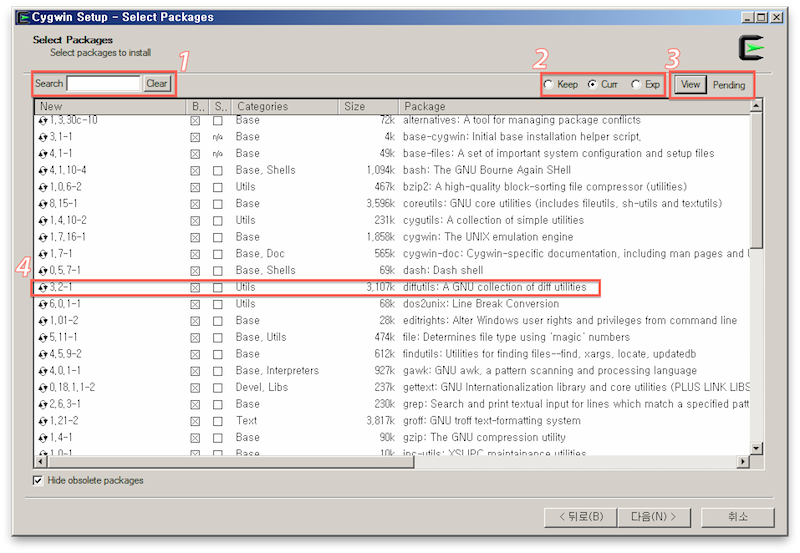
\includegraphics[width=0.95\textwidth]{img/cygwin.png}
    \label{fig:cygwin}
    \caption{설치할 \CYGWIN{} 패키지 선택}
  \end{figure}
  창 가운데에는 설치할 수 있는 \CYGWIN{} 패키지 목록입니다. 각 부분의 의미하는
  바는 다음과 같습니다.
  \begin{enumerate}
  \item 검색란입니다. 설치할 패키지 이름을 입력하면 패키지 목록이 걸러집니다.
  \item 이 버튼 중 하나를 클릭하면 패키지를 자동으로 선택합니다. ``Keep''은
    현재 \CYGWIN{} 시스템에 설치된 패키지를 그대로 유지한다는 의미입니다. 이를
    클릭하면 새로 패키지를 설치하거나 삭제하려고 선택한 사항은 모두
    취소됩니다. 그 옆의 ``Curr''은 현재 설치된 패키지 중 안정 버전으로 업데이트
    할 수 있는 것을 모두 선택하라는 의미입니다. ``Exp''은 ``Curr''과 비슷하지만
    단 안전성이 고려되지 않은 실험 버전의 패키지도 고려합니다.\footnote{여기서
      실험 버전이란 원 프로그램 개발 측(upstream)에서 실험 중이라는 것이
      아니라, 그 프로그램이 \CYGWIN{} 시스템에서 제대로 동작하는지를 \CYGWIN{}
      개발진에서 실험 중에 있다는 의미입니다. 따라서 실험 버전이어도 그것이 원
      프로그램의 최신 버전보다 옛 버전일 수도 있습니다.}
  \item 패키지 목록 형식을 지정하는 버튼입니다. 버튼을 누를 때마다
    가운데 패키지 목록이 바뀝니다. ``Pending''은 현재 설치 대상으로 지정된
    패키지만을 보여 줍니다. 설치할 패키지를 아무것도 지정하지 않더라도
    업데이트 혹은 \CYGWIN{}에 필요한 패키지가 자동으로 지정되어 있을 수도
    있습니다. ``Up To Date''는 현재 설치된 패키지 중 최신 버전의 패키지를,
    ``Not Installed''는 아직 설치되지 않은 패키지만을 보여
    줍니다. ``Category''는 패키지 목록 전체를 패키지 종류별로 분류하여,
    ``Full''은 일렬로 나열하여 보여줍니다. 참고로 ``Category''로 설정한 경우
    같은 이름의 패키지가 여러 카테고리에 중복되어 보일 수 있는데, 그렇더라도
    이는 다른 패키지가 아닌 동일한 패키지를 나타냅니다.
  \item 패키지의 정보입니다. 맨 앞은 이번 설치 과정에서 해당 패키지를 어떻게
    다룰지를 설정하는 란입니다. 클릭하면 패키지를 설치 혹은 제거하도록 지정할
    수 있습니다. ``Skip''은 이 패키지를 설치하지 않을 것임을 나타냅니다. 그 외
    숫자는 설치할 패키지 버전 정보를 나타냅니다. 여러 버전이 있다면 계속
    클릭할 때마다 버전이 바뀝니다. 중간의 ``B'' 란은 바이너리 설치 여부, ``S''
    란은 소스 코드 설치 여부입니다. 이 항목은 크게 신경쓰지 않아도 됩니다.
  \end{enumerate}
\item 이제 패키지 설치란에서 \OCAML{} 설치에 필요한 패키지를
  설치합시다. 필요한 패키지는 \texttt{curl}, \texttt{make},
  \texttt{mingw64-i686-gcc-g++}, \texttt{mingw64-i686-gcc}, \texttt{patch},
  \texttt{rlwrap}, \texttt{libreadline7} (없다면 \texttt{libreadline6}),
  \texttt{diffutils} 입니다. 각 패키지를 찾아서 맨 왼쪽란의 ``Skip'' 혹은
  버전을 클릭, 최신 버전이 설치되도록 지정합니다.
\item 설치할 패키지를 지정하였으면 ``다음''을 클릭합니다. 설치에 앞서 선택한
  패키지가 의존하는 다른 패키지도 같이 설치할 것인지 물어볼 수 있는데,
  여기서도 ``다음''을 클릭합니다. 그러면 이제 설치가 진행됩니다. 잠시 쉬다
  오세요.
\item 설치가 끝나면 바로가기를 등록할 것인지를 물어봅니다. 처음 설치하는
  것이라면 ``Add icon to Start menu''는 선택해 둡니다. 적절히 지정하고
  ``마침''을 클릭합니다.
\end{itemize}

참고로 설치가 끝나고 난 후 \texttt{setup.exe} 파일은 삭제하여도
무방합니다. 하지만 차후에 추가로 패키지를 설치해야 하는 경우에 다시 이 파일을
실행해야 하므로, 되도록 삭제하지 말고 적절한 디렉토리에 보관해 두세요. 추천하는
방법은 \texttt{setup.exe} 파일을 \CYGWIN{} 설치 디렉토리 안에 넣어두고
바로가기를 만들어 두는 것입니다.

이제 \CYGWIN{} 시스템을 사용할 수 있습니다. 바로가기를 등록해 두었다면,
시작 메뉴 내 ``Cygwin'' 프로그램 폴더 안에 ``Cygwin Terminal'' 아이콘이
추가되었을 것입니다. 이것을 클릭하면 \CYGWIN{} 시스템에서 동작하는 쉘 터미널
실행할 수 있고, 여기서 \UNIX{} 명령을 사용하면 됩니다. 만일 현재 자신이
\WINDOWS{} 어느 폴더에 있는 것인지 알고 싶다면 다음 명령을 입력하세요.

\begin{lstlisting}
$ ~explorer.exe .~
\end{lstlisting}

\CYGWIN{} 설치가 끝났으니 이제 본격적으로 \OCAML{}을 설치해 봅시다.

\paragraph{\OCAML{} 설치} \OCAML{} 설치 프로그램은 다음 주소에서
내려받을 수 있습니다. (\OCAML{} 공식 웹사이트 다운로드 페이지의 ``Binary
distributions for Microsoft Windows'' 중 ``Self installer''가 이곳에 연결됩니다).

\begin{center}
  \URL{http://protz.github.com/ocaml-installer/}
\end{center}

가운데 ``Installer for OCaml'' 링크를 내려받으면 됩니다. 내려받은 파일을
실행하여 다음과 같이 설치를 진행합니다.

\begin{itemize}
\item 설치 프로그램을 실행하면 귀여운$^?$ 낙타가 우리를 반겨줍니다. ``Next''를
  클릭합니다.
\item 설치할 프로그램 폴더를 지정하고 ``Next''를 클릭합니다.
\item \OCAML{} 라이센스를 보여줍니다. ``Next''를 클릭합니다.
\item 이제 설치할 프로그램을 선택하는 창이 열립니다. 당연히 ``OCaml''은
  선택. ``ActiveTCL''은 부가 라이브러리 중 하나인 \LABLTK{}를
  사용하는데 쓰입니다. 선택하지 않아도 무방합니다. 다음의 ``Emacs''는
  편집기인데, 일단은 선택하지 마세요. ``Emacs'' 설치 방법은
  \ref{sec:ide}절에서 따로 다룹니다. 그리고 앞에서 이미 \CYGWIN{}을
  설치했으므로 마지막 ``Cygwin''은 선택을 해제해야 합니다. 결정하였으면
  ``Next''를 클릭합니다.
\item \OCAML{} 설치 폴더를 지정합니다. 되도록 미리 주어지는
  \texttt{C:\textbackslash OCaml}을 그대로 사용하세요. 만일 다른 곳에 설치해야
  한다면 폴더명 사이에 공백이 들어가지 않도록 유의합니다. 정했으면
  ``Install''을 클릭해서 설치를 시작합니다.
\end{itemize}

설치가 모두 끝나면 \CYGWIN{} 터미널을 열어서 다음과 같이 설치한 \OCAML{}
버전을 확인해 볼 수 있습니다.

\begin{lstlisting}
$ ~ocaml -version~
The Objective Caml toplevel, version 4.00.0
$ ~ocamlc -version~
4.00.0
$ ~ocamlopt -version~
4.00.0
\end{lstlisting}

시작 메뉴 안에는 \textsf{OCamlWin}이라는 프로그램이 있는데, 이를 실행하면
\OCAML{} 탑레벨을 터미널 밖에서도 쓸 수 있습니다.

\subsubsection{문제 해결}

\WINDOWS{} 환경에서 발생할 수 있는 \OCAML{} 문제를 해결하는 방법에 대해
설명합니다.

\begin{itemize}
\item \OCAML{} 실행 시 ``\texttt{Fatal error: cannot open pervasives.cmi}'' 와
  같은 오류 발생 -- \OCAML{} 표준 라이브러리의 위치를 찾지 못하는 경우입니다.
  우선 터미널에서 다음과 같이 \OCAML{}이 사용하는 표준 라이브러리
  폴더를 확인합니다.

  \begin{lstlisting}
$ ~ocamlc -where~
c:\ocaml-3.11\lib
  \end{lstlisting}

  이 명령의 결과는 설치 과정에서 지정한 폴더 내 \texttt{lib} 폴더의 경로이어야
  합니다. (미리 지정된 폴더를 사용한 경우,
  \texttt{C:\textbackslash{}OCaml\textbackslash{}lib}). 잘못된 경로가
  출력된다면 \texttt{OCAMLLIB} 환경변수를 확인해 봐야 합니다. 우선 ``제어판'' 내
  ``시스템''을 열고 ``고급 시스템 설정''을 클릭해서 ``시스템 속성'' 창을
  엽니다. (\textsf{Windows XP}의 경우 ``시스템''만 열면 바로 열림). 여기서
  ``고급'' 탭의 ``환경 변수''를 클릭하면 시스템에 정의된 환경 변수를 찾아볼 수
  있습니다. 우리가 사용한 설치 프로그램으로 \OCAML{}을 설치하면
  \texttt{OCAMLLIB}과 같은 환경 변수는 설정할 필요없습니다. 사용자 변수,
  시스템 변수 목록에서 \texttt{OCAMLLIB}이 보이면 삭제하고 ``확인''
  클릭합니다. 그리고 나서 환경 변수 적용을 위해 터미널을 재시작해서 다시
  \OCAML{}을 실행하면 됩니다.

  만일 이 방법으로도 문제가 계속된다면 표준 라이브러리 파일에 문제가 생긴 것일 수
  있습니다. 설치 과정에서 지정한 폴더 내 \texttt{lib} 폴더가 제대로 있는지
  확인하고, \OCAML{}을 삭제한 후 재설치하세요.
\end{itemize}

%%% Local Variables: 
%%% mode: latex
%%% TeX-master: "master"
%%% End: 

\section{통합개발환경}\label{sec:ide}

이 절에서는 편리한 \OCAML{} 개발을 위한 \KOEN{통합개발환경}{integrated
  development environment} (이하 IDE)을 구축하는 방법을
소개합니다. 공식적으로는 \OCAML{} 도구는 전부 \KOEN{명령줄}{command-line}
환경만을 지원합니다. 하지만 많은 오픈소스 개발자의 노력에 힘입어 이제는
검은 화면 터미널을 떠나 어느정도 괜찮은 IDE 위에서 개발할 수 있게 되었습니다.

여기서 소개하는 IDE는 크게 두 가지로 나뉩니다. \textsf{Java} 개발 환경으로
유명한 \ECLIPSE{}에 \OCAML{} 플러그인을 장착한 것과, 전통이 있는 만능 편집기
\EMACS{}에 \OCAML{} 패키지를 장착한 것. 자신이 편한 것을 선택해서
진행합시다. 만일 \EMACS{}가 낯설다면 그나마 \ECLIPSE{}가 \EMACS{} 보다 훨씬
눈에 익숙할 테니 \ECLIPSE{} 쪽을 사용하는 것이 좋을 것입니다.

\subsection{\ECLIPSE{}와 \OCAIDE{}}

\TODO{\URL{http://www.algo-prog.info/ocaide}}

\subsection{\EMACS{}와 \TYPEREX{}}

\TODO{\URL{http://www.typerex.org}}



%%% Local Variables: 
%%% mode: latex
%%% TeX-master: "master"
%%% End: 

\section{읽을거리}\label{sec:ref}

\subsection{서적}

\TODO{서적}

\subsection{웹}

일단은 무엇보다도 다음 주소에 있는 \OCAML{} 공식 웹사이트 문서 목록을
보세요. 영어지만, 가장 중요한 내용이 담겨 있습니다. 어려워도 피하지 말고
살펴봅시다.

\begin{center}
\URL{http://caml.inria.fr/resources/doc/index.en.html}
\end{center}

질문거리가 있다면 다음 \textsf{OCaml Beginners list} 사이트를 둘러 보세요.
초보자가 놀기에 좋은 곳입니다.

\begin{center}
\URL{http://tech.groups.yahoo.com/group/ocaml\_beginners}
\end{center}

좀 더 심도깊은 질문이나 논의거리는 \textsf{The Caml Mailing List}를
사용하세요. 다음 페이지에서 구독할 수 있습니다.

\begin{center}
\URL{https://sympa-roc.inria.fr/wws/info/caml-list}
\end{center}

단 이 메일링리스트는 초보자를 위한 곳이 아닙니다. 기초적인 질문을 하면
아마 누군가 답변은 해 줄테지만, 초보가 놀 곳은 아니라는 면박도 같이 받을 수
있습니다.

메일링리스트의 수많은 메시지를 일일이 읽을 시간 없다면 다음 사이트를 둘러
보세요. 매주 메일링리스트에서 오고간 주요 논의가 요약 정리되서 올라옵니다.

\begin{center}
\URL{http://alan.petitepomme.net/cwn/}
\end{center}


\TODO{웹}

%%% Local Variables: 
%%% mode: latex
%%% TeX-master: "master"
%%% End: 


\listoftodos

\end{document}


%%% Local Variables: 
%%% mode: latex
%%% TeX-master: t
%%% End: 
